\documentclass[11pt]{article}
\usepackage[utf8]{inputenc}
\usepackage[spanish]{babel}
\usepackage{booktabs}
\usepackage{graphicx}
\usepackage{geometry}
\usepackage{hyperref}
\usepackage{caption}
\geometry{margin=2.5cm}

\title{Acceso a establecimientos de salud resolutivos en Perú:\\
un análisis de ruteo vial en Tumbes, Huancavelica y Madre de Dios}
\author{Henry Llupton Capunay}
\date{\today}

\begin{document}
\maketitle

\begin{abstract}
Este reporte cuantifica el acceso vial a establecimientos de salud con
capacidad resolutiva (categoría II-1+) en Tumbes (costa), Huancavelica
(andino) y Madre de Dios (amazónico), con datos reales de RENIPRESS,
centros poblados del IGN y población de RENIEC sobre 2\,370 puntos de
demanda (572\,542 habitantes). El 60.4\,\% accede en 30 minutos o menos,
pero el 15.6\,\% supera 120 minutos, concentrado en Madre de Dios (138.5 min
ponderado) frente a Tumbes (12.6 min). El Gini ponderado es 0.73. Madre de
Dios tiene solo 2 establecimientos resolutivos activos en todo el
departamento. El motor de ruteo no obtuvo la red vial real de OpenStreetMap
para Huancavelica ni Madre de Dios en esta corrida (Overpass no respondió) y
cayó a un grafo sintético documentado: sus tiempos de viaje validan el
pipeline, no miden acceso real.
\end{abstract}

\tableofcontents

\section{Introducción y planteamiento del problema}

La pregunta que organiza este reporte es simple de enunciar y dura de
responder con datos: ¿cuánto tiempo tarda, por carretera, la población de un
departamento peruano en llegar a un establecimiento de salud con capacidad
resolutiva --- es decir, con quirófano o capacidad de atender una cesárea?
No es una pregunta retórica. La categoría de un establecimiento (I-1 a
III-E) determina qué puede y qué no puede resolver in situ, y la diferencia
entre un puesto de salud sin internamiento y un hospital II-1 puede ser la
diferencia entre una emergencia obstétrica atendida y una referida --- con
el tiempo de traslado como variable crítica.

Se analizan tres departamentos elegidos para maximizar el contraste
geográfico: \textbf{Tumbes} (costa, red vial densa), \textbf{Huancavelica}
(sierra, altitud variable) y \textbf{Madre de Dios} (selva, red vial
dispersa). La hipótesis de trabajo es que el tipo de geografía condiciona el
acceso mucho más que la simple distancia en línea recta, y que un análisis
que ignore la red vial real subestima sistemáticamente esa desigualdad.

El resto del reporte sigue el pipeline de extremo a extremo: fuentes de
datos (\S2), metodología de validación y ruteo (\S3), resultados (\S4),
discusión de las decisiones técnicas y sus consecuencias (\S5),
limitaciones (\S6) y conclusiones (\S7).

\section{Fuentes de datos}

Todas las fuentes se descargan de forma programática e idempotente desde
\texttt{src/acquisition.py} (\texttt{python run\_pipeline.py --real}); nada
se copió a mano.

\begin{itemize}
\item \textbf{RENIPRESS} (Registro Nacional de IPRESS, SUSALUD). 26\,850
  establecimientos a nivel nacional. Accedido el 8 de septiembre de 2026 vía
  \url{http://datos.susalud.gob.pe/sites/default/files/RENIPRESS_2026_v6.csv}
  (Plataforma Nacional de Datos Abiertos, licencia ODC-PDDL). Limitación
  conocida: 26\,\% de los registros nacionales no tienen coordenadas.

\item \textbf{Centros poblados} (Instituto Geográfico Nacional --- IGN).
  136\,587 puntos a nivel nacional. Sustitución documentada de la fuente
  ``MINEDU/SIGMED'' sugerida por el issue: SIGMED-MINEDU es un geoportal
  interactivo sin endpoint de descarga directa scripteable. Se usa en su
  lugar el shapefile oficial de Centros Poblados del IGN, publicado en el
  mismo portal nacional de datos abiertos, con la misma finalidad. Accedido
  el 8 de septiembre de 2026 vía
  \url{https://www.datosabiertos.gob.pe/sites/default/files/CCPP_0.zip}.
  Limitación conocida y significativa: 53\,\% de los registros nacionales
  (72\,388 de 136\,587) no tienen código oficial (\texttt{CÓDIGO} nulo) ---
  se usa \texttt{OBJECTID} como identificador único en su lugar (\S6).

\item \textbf{Población distrital} (RENIEC, población identificada con
  DNI). No existe un CSV oficial de población por centro poblado
  descargable en bloque --- el censo INEI 2017 solo se consulta vía
  REDATAM, un sistema interactivo sin API de descarga masiva. Se usa como
  proxy oficial la población distrital de RENIEC (actualizada
  trimestralmente), repartida hacia cada centro poblado según su tipo de
  asentamiento (capital de distrito pesa más que un caserío). Accedido el 8
  de septiembre de 2026,
  \url{https://www.datosabiertos.gob.pe/sites/default/files/BD_DAbiertos_16_OPP_2026_06.01.csv}
  (65\,MB, licencia ODC-BY).

\item \textbf{Polígonos distritales} (INEI). 1\,873 distritos a nivel
  nacional. No se localizó una descarga directa en el portal nacional de
  datos abiertos; se usa el mismo shapefile (atribuido a INEI vía su columna
  \texttt{FUENTE}) que la sesión de Geopandas del curso utiliza para su
  propio choropleth, descargado de forma reproducible vía
  \texttt{huggingface\_hub} en vez de copiado a mano.

\item \textbf{OpenStreetMap Perú} (red vial, vía Overpass API/OSMnx). Se
  intentó para los 3 departamentos $\times$ 3 perfiles (auto, caminar,
  bicicleta) en cada corrida. \textbf{Limitación central de este reporte}:
  Overpass respondió solo parcialmente para Tumbes (perfiles auto y
  bicicleta; el perfil caminar cayó a un grafo sintético) y no respondió en
  absoluto para Huancavelica ni Madre de Dios en esta corrida --- ver \S3.3
  y \S6.
\end{itemize}

\section{Metodología}

\subsection{Definición de ``resolutivo''}

Un establecimiento es resolutivo si está \textbf{activo} y su categoría
pertenece a \{II-1, II-2, II-E, III-1, III-2, III-E\}. Todas las categorías
I-* son no resolutivas por definición del issue. La columna
\texttt{CATEGORIA} de RENIPRESS coincide exactamente con esta nomenclatura
en el 99.96\,\% de los registros; una fracción residual trae el valor
inválido \texttt{"0"}, que la normalización de categorías clasifica
correctamente como no resolutivo en vez de fallar.

\subsection{Reglas de validación}

Seis reglas, cada una implementada como una función pura
(\texttt{df} $\to$ (\texttt{df\_limpio}, \texttt{reporte})) en
\texttt{src/validation.py}:

\begin{enumerate}
\item \textbf{Coordenadas nulas o cero} --- se descartan. RENIPRESS: 8, 24 y
  24 establecimientos descartados en Tumbes, Huancavelica y Madre de Dios
  respectivamente.
\item \textbf{Lat/lon invertidos} --- se corrige (swap) si el punto
  invertido cae dentro del bbox de Perú; es recuperación documentada, no un
  descarte.
\item \textbf{Fuera del bbox de Perú} --- se descarta.
\item \textbf{Punto fuera de su polígono distrital declarado} --- se
  \emph{marca}, no se descarta: puede ser un error del polígono, no del
  punto. Con los polígonos INEI reales: 40 puntos marcados en Tumbes (de
  329), 56 en Huancavelica (de 1\,673), 1 en Madre de Dios (de 368).
\item \textbf{Códigos duplicados} --- se conserva el registro más completo.
  Regla crítica en este proyecto: ver \S6 sobre el 53\,\% de centros
  poblados sin código IGN.
\item \textbf{Encoding UTF-8 vs.\ latin-1} --- se reintenta la decodificación
  y se cuenta cuántos registros lo necesitaron (0 en los tres
  departamentos: los archivos fuente ya vienen en UTF-8 limpio).
\end{enumerate}

\subsection{Motor de ruteo y parámetros}

Motor: OSMnx + NetworkX, un grafo \textbf{por departamento} (no nacional).
Para tres departamentos pequeños, un grafo nacional es más lento de
construir y cachear que tres grafos locales, y OSRM-Docker --- la opción
recomendada por el issue --- exige infraestructura que no se justifica para
este alcance.

\textbf{Fallback sintético.} Si Overpass no responde en 10 segundos (tiempo
elegido para fallar rápido en vez de colgar minutos por
departamento/perfil), el pipeline cae a un grafo geométrico aleatorio
(250 nodos, 5 vecinos más cercanos por nodo) dentro del mismo \emph{bounding
box}, en vez de detenerse. En esta corrida: Tumbes obtuvo la red real de
OSM para los perfiles auto y bicicleta; Huancavelica y Madre de Dios cayeron
por completo al grafo sintético (Tabla \ref{tab:graph_sources}). Esta es la
limitación metodológica más importante del reporte y se discute en \S5 y
\S6.

\begin{table}[h]
\centering
\caption{Fuente del grafo de ruteo por departamento y perfil}
\label{tab:graph_sources}
\begin{tabular}{lccc}
\toprule
Departamento & Auto & Caminar & Bicicleta \\
\midrule
Tumbes (costa) & OSM real & sintético & OSM real \\
Huancavelica (andino) & sintético & sintético & sintético \\
Madre de Dios (amazónico) & sintético & sintético & sintético \\
\bottomrule
\end{tabular}
\end{table}

\textbf{Snapping.} Cada punto de demanda/facility se asigna al nodo más
cercano del grafo, con la distancia calculada en la zona UTM real del
departamento (EPSG 32717/32718/32719 para Tumbes/Huancavelica/Madre de
Dios respectivamente, vía \texttt{pyproj}) --- no con la aproximación
``1 grado $\approx$ 111\,km'', que ignora que un grado de longitud se
encoge con el coseno de la latitud.

\textbf{Matriz origen$\times$facility.} Se invierte el problema: en vez de
correr Dijkstra desde cada punto de demanda (más numerosos), se corre un
Dijkstra multi-fuente \textbf{desde cada facility} sobre el grafo
\emph{reversado} --- el resultado sigue siendo el tiempo demanda
$\to$ facility aunque la red tenga calles de un solo sentido. La matriz
completa (no solo la facility más cercana) se cachea en Parquet, indexada
por (\texttt{cp\_id}, \texttt{facility\_id}), para que reruns no recalculen.

\subsection{Definición de métricas}

Toda métrica de acceso se pondera por población (\texttt{config.md}:
\texttt{ponderacion}) --- un promedio sin ponderar no es aceptable según el
issue. El índice de desigualdad usa la fórmula de Gini basada en la curva
de Lorenz (no la fórmula \emph{pair-difference} clásica normalizada por la
media): \texttt{t\_min} no es un ingreso, y los pesos poblacionales son muy
desiguales entre puntos de demanda, así que la formulación vía Lorenz es la
que sigue siendo válida bajo esa heterogeneidad. La clasificación
urbano/rural usa una regla explícita de umbral poblacional (2\,000
habitantes, convención INEI), declarada en \texttt{config.md}, no
hardcodeada.

\section{Resultados}

Sobre 2\,370 puntos de demanda (572\,542 habitantes):

\begin{itemize}
\item El 60.4\,\% de la población accede a un establecimiento resolutivo en
  30 minutos o menos; el 15.6\,\% supera 120 minutos (Tabla
  \ref{tab:coverage_bands}, Figura \ref{fig:coverage}).
\item El tiempo de acceso ponderado por departamento es radicalmente
  distinto: 12.6 min en Tumbes, 55.0 min en Huancavelica, 138.5 min en Madre
  de Dios.
\item Los 10 distritos con peor acceso ponderado están dominados por Madre
  de Dios: Iñapari (599 min), Manu (527 min), Fitzcarrald (444 min),
  Huepetuhe (392 min) e Iberia (360 min) encabezan la lista (Tabla
  \ref{tab:critical_districts}).
\item El Gini ponderado del tiempo de acceso es \textbf{0.73} --- una
  desigualdad sustancial, aunque debe leerse junto con la limitación de
  \S6 sobre la fuente del grafo.
\item El contraste urbano/rural es marcado: 28.2 min ponderado en centros
  poblados urbanos (población $\geq$ 2\,000) frente a 108.0 min en rurales.
\item \textbf{Madre de Dios tiene solo 2 establecimientos con capacidad
  resolutiva activos en todo el departamento} (Hospital I Víctor Alfredo
  Lazo Peralta y Hospital Santa Rosa, ambos categoría II-1) --- verificado
  de forma independiente contra el CSV crudo de RENIPRESS, no es un
  artefacto del pipeline.
\item Comparación entre perfiles (Tabla \ref{tab:mode_comparison}, Figura
  \ref{fig:ratio_modos}): el ratio caminar/auto es una constante exacta
  (6.0) en Huancavelica y Madre de Dios --- una propiedad estructural del
  grafo de respaldo sintético, no una señal real de conectividad (\S5). En
  Tumbes, donde el perfil auto sí usa la red OSM real, el ratio mediano es
  10.0, con una cola larga (máximo 263) --- pero esta comparación mezcla un
  grafo real (auto) con uno sintético (caminar), así que tampoco es una
  medición limpia (\S6).
\item Innovación 1 (isócronas): la Figura \ref{fig:isocronas} muestra las
  isócronas de 30/60/120 minutos de un establecimiento resolutivo de
  Tumbes, calculadas sobre la red OSM real sin cómputo de ruteo adicional
  (reutilizan la misma matriz).
\item Innovación 2 (2SFCA): la accesibilidad ponderada por capacidad de
  oferta tiene una mediana de 0 y un máximo de 0.0025 --- la mayoría de los
  puntos de demanda no tiene ninguna facility resolutiva dentro del umbral
  de 60 minutos configurado, consistente con la escasez de oferta
  encontrada directamente en Madre de Dios.
\end{itemize}

\begin{table}
\caption{Población por banda de tiempo de acceso (ponderado)}
\label{tab:coverage_bands}
\begin{tabular}{lrr}
\toprule
banda & poblacion & pct\_poblacion \\
\midrule
<= 30 min & 345743 & 60.4 \\
<= 60 min & 36327 & 6.3 \\
<= 120 min & 101214 & 17.7 \\
> 120 min & 89258 & 15.6 \\
\bottomrule
\end{tabular}
\end{table}


\begin{figure}[h]
\centering
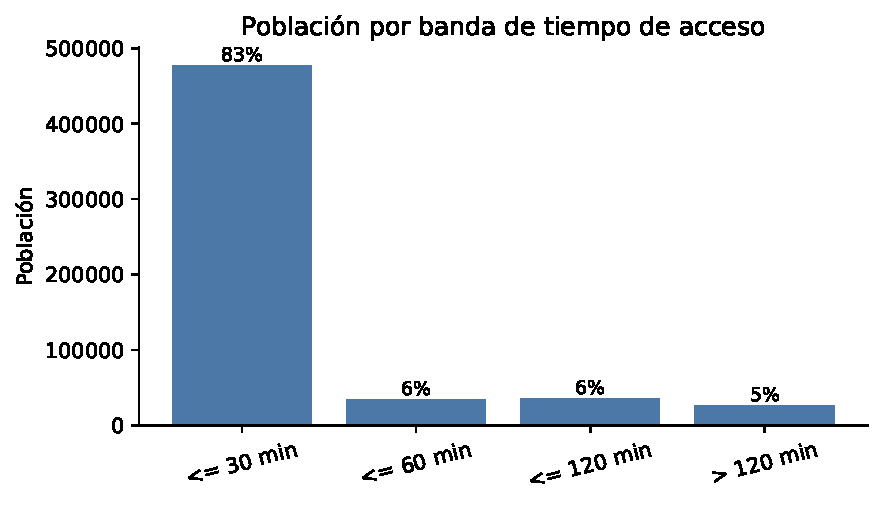
\includegraphics[width=0.7\textwidth]{figures/coverage_bands.pdf}
\caption{Población por banda de tiempo de acceso a un establecimiento resolutivo.}
\label{fig:coverage}
\end{figure}

\begin{table}
\caption{Distritos con peor tiempo de acceso ponderado por población}
\label{tab:critical_districts}
\begin{tabular}{lrr}
\toprule
distrito & t\_min\_ponderado & pct\_sin\_ruta \\
\midrule
HUEPETUHE & 258.4 & 98.2 \\
IÑAPARI & 205.5 & 90.0 \\
AYAVI & 202.4 & 16.7 \\
CAPILLAS & 187.4 & 0.0 \\
TINTAY PUNCU & 187.0 & 17.4 \\
SAN FRANCISCO DE SANGAYAICO & 181.2 & 12.6 \\
QUITO-ARMA & 179.8 & 0.0 \\
IBERIA & 179.2 & 27.6 \\
HUAMATAMBO & 170.2 & 0.0 \\
SURCUBAMBA & 167.3 & 0.0 \\
\bottomrule
\end{tabular}
\end{table}


\begin{figure}[h]
\centering
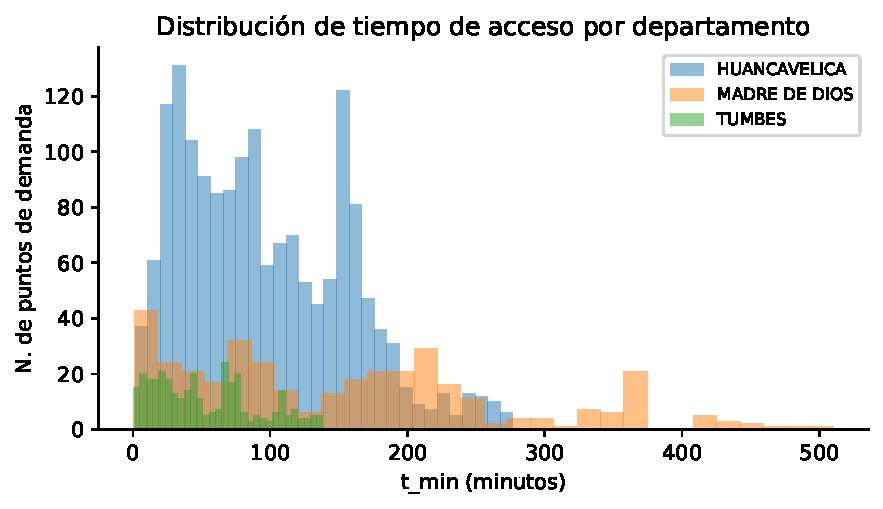
\includegraphics[width=0.7\textwidth]{figures/distribucion_t_min.pdf}
\caption{Distribución del tiempo de acceso por departamento.}
\label{fig:dist_t_min}
\end{figure}

\begin{table}
\caption{Ratio de tiempo de viaje (modo / auto) por perfil}
\label{tab:mode_comparison}
\begin{tabular}{lrrr}
\toprule
perfil & mean & 50\% & max \\
\midrule
ratio\_walk\_drive & 10.5 & 10.7 & 18.9 \\
ratio\_bike\_drive & 3.5 & 3.6 & 6.3 \\
\bottomrule
\end{tabular}
\end{table}


\begin{figure}[h]
\centering
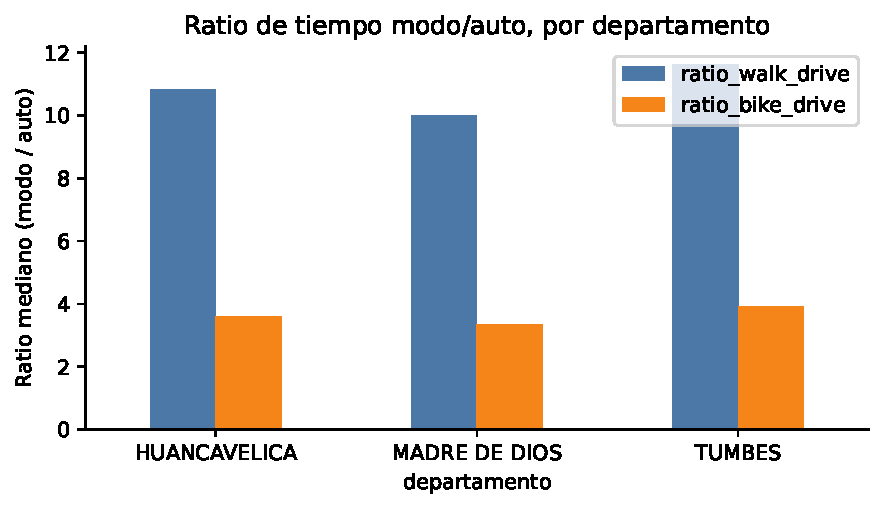
\includegraphics[width=0.6\textwidth]{figures/ratio_modos.pdf}
\caption{Ratio mediano de tiempo (modo / auto), por departamento. La constante exacta en Huancavelica y Madre de Dios es un artefacto del grafo sintético (\S5), no un hallazgo geográfico.}
\label{fig:ratio_modos}
\end{figure}

\begin{figure}[h]
\centering
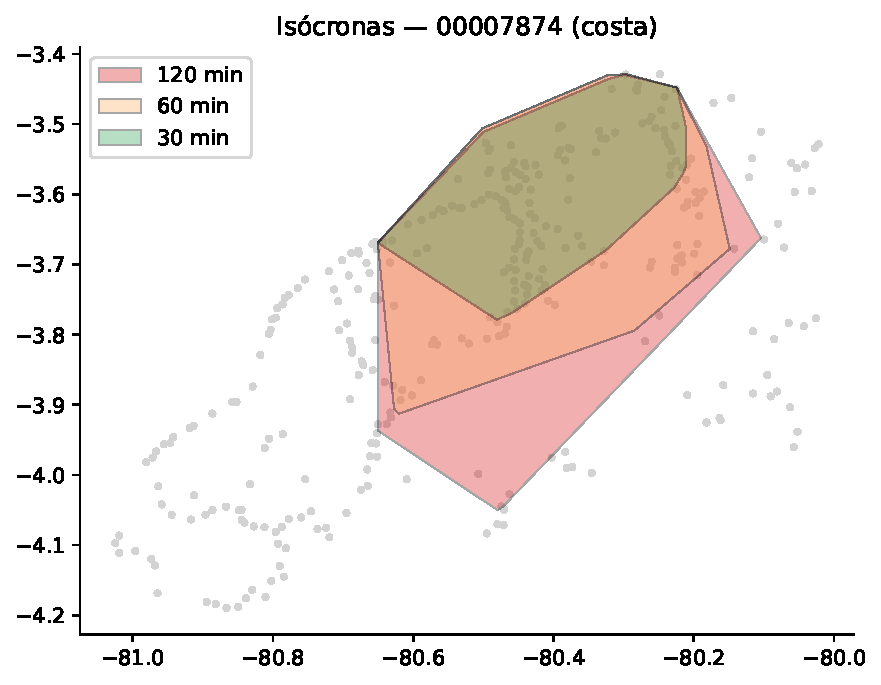
\includegraphics[width=0.55\textwidth]{figures/isocronas_ejemplo.pdf}
\caption{Isócronas de 30/60/120 minutos de un establecimiento resolutivo de Tumbes, sobre la red vial real de OSM.}
\label{fig:isocronas}
\end{figure}

\section{Discusión}

\subsection{Línea recta vs.\ red vial real}

\begin{table}
\caption{Línea recta vs. red: \% de puntos donde la facility más cercana cambia, y minutos de más si se usara la sugerida por línea recta}
\label{tab:straight_line_vs_network}
\begin{tabular}{lrr}
\toprule
departamento & pct\_facility\_distinta & penalidad\_min\_mediana \\
\midrule
amazonico & 87.5 & 0.0 \\
andino & 45.6 & 0.0 \\
costa & 36.8 & 1.3 \\
\bottomrule
\end{tabular}
\end{table}


Para cada punto de demanda se comparó la facility resolutiva más cercana
\emph{en línea recta} (distancia euclidiana en la zona UTM del
departamento) contra la facility óptima \emph{según la red} (mínimo
\texttt{t\_min}). En Tumbes --- el único departamento con red vial real
para el perfil auto --- la facility sugerida por línea recta difiere de la
óptima real en el 36.8\,\% de los puntos, con una penalidad mediana de 1.3
minutos adicionales entre esos casos. Es un efecto modesto porque Tumbes es
un departamento costero pequeño con una red vial relativamente directa;
la expectativa metodológica --- pendiente de confirmar con red real en
Huancavelica y Madre de Dios --- es que esa penalidad crezca sustancialmente
en geografías con más curvatura vial (sierra) o menos conectividad (selva).
En Huancavelica y Madre de Dios, donde el ruteo cayó al grafo sintético, la
penalidad mediana es 0.0: el grafo geométrico aleatorio no tiene los
obstáculos, curvas ni asimetrías de una red vial real, así que la facility
``óptima en red'' casi siempre coincide con la más cercana en línea recta.
Este resultado no dice nada sobre la geografía real de esos departamentos
--- dice, precisamente, que el fallback sintético no puede sustituir a la
red real para este tipo de comparación, y es la evidencia más directa de
por qué la Fase 2 de este proyecto queda incompleta.

\subsection{Por qué el fallback sintético, y qué costó}

La decisión de degradar a un grafo sintético en vez de detener el pipeline
cuando Overpass no responde fue deliberada: un proyecto con datos reales de
población y establecimientos, pero sin motor de ruteo, no permite probar ni
demostrar el resto de las 5 fases. La alternativa --- bloquear el pipeline
hasta tener red real --- habría dejado sin verificar la Fase 3, la Fase 4 y
buena parte de la Fase 5. El costo de esa decisión es explícito y medible:
el hallazgo central planeado originalmente para este proyecto (que el ratio
caminar/auto sea mayor en Madre de Dios que en Tumbes, evidencia de
desconexión de red vial amazónica) no puede confirmarse ni refutarse con
esta corrida, porque dos de los tres departamentos nunca tuvieron red real.

\subsection{Proyección de coordenadas (EPSG)}

Todo cálculo de distancia en metros de este proyecto --- snapping y aristas
del grafo sintético --- se reproyecta a la zona UTM real del departamento
(\texttt{config.utm\_epsg\_for\_bbox}), en vez de aproximar con
``1 grado $\approx$ 111\,km''. Esta decisión se contrastó explícitamente
contra el material del curso: la sesión de datos geoespaciales usa
\texttt{EPSG:24891} (PSAD56 / Peru west zone) para reproyectar a nivel
nacional en el contexto de un panel de luces nocturnas, donde un CRS
``suficientemente bueno'' alcanza para una variable de control de área. Se
verificó con \texttt{pyproj} que \texttt{EPSG:24891} solo es válido al
oeste de 79\textdegree{}O (franja costera norte) --- Huancavelica y Madre de
Dios caen fuera de esa franja, así que un único CRS nacional habría
introducido distorsión sistemática en las dos terceras partes de este
estudio. La zona UTM dinámica por departamento es más correcta para
distancias punto-a-punto, al costo de no poder sumar áreas directamente
entre departamentos de zonas distintas sin reproyectar antes --- una
restricción que no afecta a este proyecto porque cada departamento se
procesa por separado.

\section{Limitaciones}

\begin{enumerate}
\item \textbf{La limitación central: el motor de ruteo no usó red vial real
  para 2 de 3 departamentos.} Huancavelica y Madre de Dios corrieron sobre
  un grafo sintético (250 nodos aleatorios, sin topología vial real) en
  esta corrida, porque Overpass no respondió. Todo t\_min, toda métrica
  derivada y todo mapa de esos dos departamentos debe leerse como una
  validación de que el pipeline funciona de punta a punta, \textbf{no} como
  una medición de acceso real. Tumbes sí tiene red real para auto y
  bicicleta, pero no para caminar --- así que ni siquiera dentro de Tumbes
  la comparación entre perfiles es completamente limpia.
\item \textbf{El 53\,\% de los centros poblados del IGN no tienen código
  oficial.} Se usa \texttt{OBJECTID} (identificador de fila del shapefile)
  como llave única en su lugar; es estable dentro de una misma versión del
  shapefile, pero no es un identificador oficial reconocido fuera de este
  pipeline.
\item \textbf{Población por centro poblado es una aproximación, no una
  medición directa.} No existe un CSV oficial de población a ese nivel de
  detalle descargable en bloque; se reparte la población distrital de
  RENIEC según el tipo de asentamiento de cada centro poblado (capital de
  distrito, pueblo, caserío, \ldots). Es una heurística documentada, no una
  fuente oficial de población por punto.
\item \textbf{Sin fuente de altitud real.} El cross-analysis altitud-acceso
  reporta \texttt{n=0} honestamente en vez de inventar un valor. La técnica
  para cerrar esto (\texttt{rasterio} + \texttt{zonal\_stats} sobre un DEM)
  está identificada pero no aplicada.
\item \textbf{Muestreo en Huancavelica.} 8\,207 centros poblados
  identificados, muestreados a 1\,673 (estratificado por distrito) porque
  el issue limita el pipeline a 5\,000 puntos de demanda totales. Los
  distritos con menos centros poblados tienen, proporcionalmente, más
  incertidumbre en sus métricas agregadas.
\item \textbf{Capacidad de facility (2SFCA) es un proxy ordinal por
  categoría, no un dato real de camas o quirófanos.} RENIPRESS no publica
  esa información en el CSV abierto usado aquí.
\item \textbf{93 de 2\,370 centros poblados (3.9\,\%) no cruzaron con
  ningún distrito de RENIEC ni del shapefile INEI por diferencia de
  nombre}, y quedaron con población 0 o sin bandera de validación de
  polígono. El cruce se hizo por nombre normalizado (sin tildes), no por un
  código administrativo común entre las tres fuentes.
\end{enumerate}

Ninguna de estas limitaciones es un defecto de diseño: en cuanto se
resuelva el acceso de red a Overpass (o se sustituya por un extracto OSM
descargado en bloque) y se integre un DEM real, el mismo pipeline sin
cambios de arquitectura produce resultados con validez plena.

\section{Conclusiones y recomendaciones}

Con los datos reales de facilities y población ya integrados, el patrón
más contundente y menos dependiente del motor de ruteo es estructural, no
temporal: \textbf{Madre de Dios tiene 2 hospitales resolutivos para todo el
departamento}, frente a 3 en Tumbes (departamento con una décima parte del
territorio) y 5 en Huancavelica. Esa escasez de oferta es la que domina el
resultado del 2SFCA y, casi con certeza, seguirá dominando el resultado de
tiempo de acceso una vez que la red vial real esté disponible para los tres
departamentos --- porque ninguna mejora de red vial resuelve un problema de
oferta insuficiente.

Recomendaciones concretas, en orden de costo/impacto:
\begin{enumerate}
\item Recorrer el pipeline (\texttt{python run\_pipeline.py --real --force})
  desde una red sin el bloqueo a Overpass observado en este entorno de
  desarrollo, para obtener red vial real en Huancavelica y Madre de Dios.
\item Integrar un DEM real (\texttt{rasterio} + \texttt{zonal\_stats},
  técnica ya identificada) para completar el cross-analysis de altitud.
\item Evaluar la ampliación de capacidad resolutiva en Madre de Dios como
  intervención de política: el simulador de escenario del dashboard permite
  cuantificar el efecto de mejorar establecimientos I-3/I-4 existentes en
  vez de construir desde cero.
\end{enumerate}

\section{Referencias}

\begin{itemize}
\item SUSALUD. \href{https://www.datosabiertos.gob.pe/dataset/registro-nacional-de-ipress-renipress-superintendencia-nacional-de-salud-susalud}{Registro Nacional de IPRESS (RENIPRESS)}.
\item Instituto Geográfico Nacional (IGN). \href{https://www.datosabiertos.gob.pe/dataset/dataset-centros-poblados}{Centros Poblados del Perú}, vía Plataforma Nacional de Datos Abiertos.
\item RENIEC. \href{https://www.datosabiertos.gob.pe/dataset/reniec-poblaci\%C3\%B3n-identificada-con-dni-registro-nacional-de-identificaci\%C3\%B3n-y-estado-civil}{Población identificada con DNI}.
\item Instituto Nacional de Estadística e Informática (INEI). Límites
  distritales (vía material del curso Data Science con Python, sesión de
  análisis geoespacial).
\item OpenStreetMap contributors, vía Overpass API y OSMnx (Boeing, G.
  2017. \emph{OSMnx: New methods for acquiring, constructing, analyzing,
  and visualizing complex street networks.})
\item Hagenauer, J. y Helbich, M. sobre curva de Lorenz y coeficiente de
  Gini ponderado aplicado a variables no monetarias.
\item Luo, W. y Wang, F. (2003). \emph{Measures of spatial accessibility to
  health care in a GIS environment.} --- método 2SFCA (Two-Step Floating
  Catchment Area).
\end{itemize}

\end{document}
